% This is samplepaper.tex, a sample chapter demonstrating the
% LLNCS macro package for Springer Computer Science proceedings;
% Version 2.20 of 2017/10/04
%
\documentclass[runningheads]{llncs}
%
\usepackage{xcolor}
\usepackage{graphicx}
\usepackage{makecell}
\usepackage{textcomp}
%\usepackage{amsmath,amssymb,amsfonts}
\usepackage{hyperref}
\usepackage{algorithm,algorithmic}
\usepackage{wrapfig}
\usepackage{mathtools}
\usepackage{tabularx}
\usepackage{etoolbox}

% Used for displaying a sample figure. If possible, figure files should
% be included in EPS format.
%
% If you use the hyperref package, please uncomment the following line
% to display URLs in blue roman font according to Springer's eBook style:
% \renewcommand\UrlFont{\color{blue}\rmfamily}

\renewcommand{\baselinestretch}{0.975}

\begin{document}
%
%\title{Automated Formal Synthesis of Optimal Sizing for Stand-alone Solar Photovoltaic Systems\thanks{Supported by Newton Fund (ref. 261881580) and FAPEAM (Amazonas State Foundation for Research Support, calls 009/2017 and PROTI Pesquisa 2018).}}
\title{Synthesis of Solar Photovoltaic Systems: Optimal Sizing Comparison\thanks{Supported by Newton Fund (ref. 261881580) and FAPEAM (Amazonas State Foundation for Research Support, calls 009/2017 and PROTI Pesquisa 2018).}}
%
%\titlerunning{Abbreviated paper title}
% If the paper title is too long for the running head, you can set
% an abbreviated paper title here
%
\author{Alessandro Trindade\inst{1} \and Lucas Cordeiro\inst{2}} %\orcidID{0000-0001-8262-2919} \orcidID{0000-0002-6235-4272}
%
\authorrunning{A. Trindade and L. Cordeiro}
% First names are abbreviated in the running head.
% If there are more than two authors, 'et al.' is used.
%
\institute{Federal University of Amazonas, Brazil, \email{alessandrotrindade@ufam.edu.br} \and
University of Manchester, UK, \email{lucas.cordeiro@manchester.ac.uk}}
\maketitle       % typeset the header of the contribution


\begin{abstract}
\textcolor{blue}{In the current scenario, energy demand rises by 1.3\% each year to 2040, and photovoltaic (PV) systems} have emerged as an alternative to the fossil or nuclear fuel energy generation. The use of formal methods for PV systems is a new subject with significant research spanning only five years. Here we develop and evaluate \textcolor{blue}{an} automated synthesis approach to obtain optimal sizing \textcolor{blue}{of PV systems based on Life Cycle Cost (LCC) analysis, where only the acquisition cost is considered in the model. The optimal solution is the lowest cost from a list of equipment that meets the electrical demands from a house}. 
We propose a variant of the counterexample guided inductive synthesis (CEGIS) approach with two phases linking the technical and cost analysis. We advocate that \textcolor{blue}{our technique} has various advantages if compared to off-the-shelf optimization tools available in the market. Experimental results from seven case studies demonstrate that we can produce an optimal solution within an acceptable run-time; different software verifiers are evaluated to check performance and soundness. We also compare our approach with a commercial tool specialized in PV systems optimization. Both results are validated with commercial design software; furthermore, some real PV systems comparison are used to show our approach effectiveness. 
\keywords{Formal Synthesis \and Software Verification \and Solar Photovoltaic Systems \and Cyber-Physical Systems.}
\end{abstract}

%%%%%%%%%%%%%%%%%%%%%%%%%%%%%%%%%%%%%%%%%%%%%%%%%%%%%%%%
\section{Introduction}
%%%%%%%%%%%%%%%%%%%%%%%%%%%%%%%%%%%%%%%%%%%%%%%%%%%%%%%%

Lack of access to clean and affordable energy is considered a core dimension of poverty~\cite{Hussein2012}. Progress has been made worldwide; \textcolor{blue}{in particular, in 2017, the number of people without electricity access fell below $1$ billion for the first time}~\cite{IEAweo2018}. The share of people without access to electricity from Africa is 58\%, while 19\% of the share comes from developing Asia, and 31\% from Latin America~\cite{IEAweo2018}. Numbers from Brazil show the aim to electrify 270 isolated areas and 2.7 million people by 2023~\cite{EPE2018}. 
There exists a close relationship between the lack of energy and the low HDI (Human Development Index) of those localities~\cite{Coelho}. It follows that increased access to energy allows economic growth and poverty alleviation \cite{Karekesi}. To provide electricity for all, decentralized systems led by solar photovoltaic (PV) in off-grid and mini-grid systems will be the lowest-cost solution for three-quarters of the connections needed~\cite{Hussein2012}. 

To evaluate \textcolor{blue}{or to obtain the optimal sizing of} a PV system, there exist various specialized tools, e.g., RETScreen~\cite{Pradhan} and HOMER~\cite{Swarnkar}; and even general-purpose tools, e.g., MATLAB/Simulink~\cite{Gow1999}. However, these tools are based on simulation; \textcolor{blue}{they have the drawback of incomplete coverage of design-space} since verification of all possible combinations, and potential failures of a system are \textcolor{blue}{not feasible}~\cite{ClarkeHV18}. 

However, the industry demands the \textcolor{blue}{design solution to be the optimum, considering equipment manufacturers and models available on the market and not just minimum or maximum values of current or power for the optimized items. It is necessary to evaluate the electrical compatibility among the equipment as well. This evaluation can only be achieved with specialized PV optimization software. Therefore, the optimal solution is the lowest cost from a list of equipment that meets the electrical demands of a house. It is based on Life Cycle Cost (LCC) analysis \textcolor{red}{add citation}, where the acquisition and replacement cost are considered over a specific period in years.}

Optimization of PV systems is not a recent topic; since the 1990s, different techniques using different criteria to find ultimate combinations for design parameters, based on intuitive, numerical, and analytical methods, were proposed and developed~\cite{Alsadi2018}. \textcolor{blue}{Concerning the use of automated verification or synthesis to electrical systems, we can mention that} in $2015$, an automated simulation-based verification technique was applied to verify the correctness of power system protection settings~\cite{Sengupta2015}. \textcolor{blue}{In $2017$, it was suggested the application of formal methods to verify and control the behavior of devices in a smart grid (e.g.,~\cite{Abate2017})}. In $2018$, a verification methodology was applied to PV panels and its distributed power point tracking~\cite{Driouich2018}. Lastly, in $2019$, an automated verification methodology was proposed to validate \textcolor{blue}{the sizing of} stand-alone solar PV systems~\cite{TrindadeCordeiro19}. \textcolor{blue}{However, \textit{formal methods and its application to synthesize PV systems are not explored in literature, mainly because it requires background and experience in computer science and PV systems, which is not common}}.

Here we developed a variant of the counterexample guided inductive synthesis (CEGIS)~\cite{AbateCAV2018} technique for synthesizing optimal sizing of stand-alone PV systems. If we provide a correctness specification $\sigma$, our method uses that as a starting point and then iteratively produces a sequence of candidate solutions that satisfy $\sigma$, related to power reliability. In particular, on each iteration, we synthesize the sizing of stand-alone PV systems, but that may not achieve the lowest cost. The candidate solution is then verified via software model checking with a lower bound that serves as the minimum cost of reference. If the verification step does not produce a counterexample, then the lower bound is adjusted; otherwise, we have achieved an optimal PV sizing.

Our work makes three significant contributions to advance the state-of-the-art in PV optimal sizing. First, the use of automated software verification in PV systems was uncommon in recent prior studies; we have shown that formal methods can detect various errors in PV systems designed by existing commercial tools~\cite{TrindadeCordeiro19}. The application of software verification to synthesize PV sizing is novel, thereby leading to more accurate results than existing commercial tools. Second, we evaluate our approach using different state-of-the-art software verifiers to obtain the best performance in our verification back-end for synthesizing optimal PV systems. We compare that to HOMER Pro optimization, with the results being validated with accurate commercial design software called PVsyst. Lastly, we discuss the challenges of applying software verification to PV systems and reflect on lessons learned from this experience.

\vspace{-2ex}

%-----------------------------------------------------------
\section{Background}
\label{sec:AutomatedVerification}
%-----------------------------------------------------------
\vspace{-1ex}

\textcolor{blue}{Fig.~\ref{fig:optimization} illustrates how to obtain the optimal sizing of a stand-alone PV system using the manual or simulation techniques and the proposed synthesis technique}. Note that the input information is the same for all the methods: weather data, price information, design requirements, as load curve and power demand, and design assumptions. \textcolor{blue}{However, when using automated synthesis, we also define the bound $k$ to restrict the design-space search}. Here we start with a low bound $k$ and incrementally increase it to avoid time and memory constraints on our verification engine. Therefore, the proper choice of $k$ is essential to this method.
%
\begin{figure}[h]
\fbox{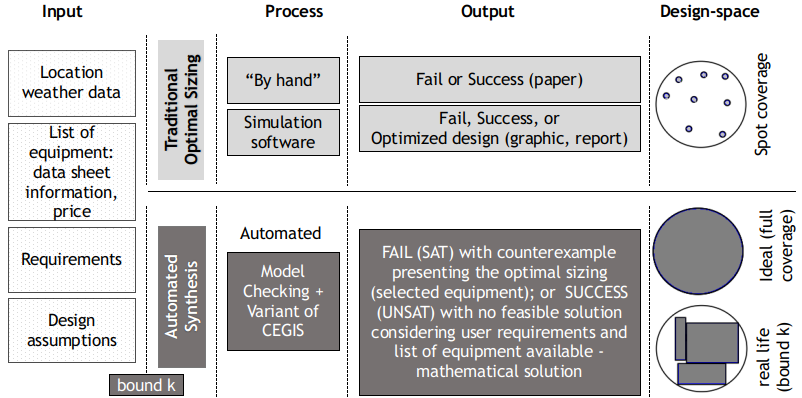
\includegraphics[width=0.9\textwidth]{optimalsizingprocess4}}
\centering
\caption{Comparison of optimal sizing methods.}
\label{fig:optimization}
\end{figure}

The techniques (manual, simulation, and automated synthesis) produce either a SUCCESS or FAIL result, thereby considering a feasible technical solution with the lowest cost. On the one hand, when done by simulation, we get a report or graphical result; on the other hand, the automated synthesis technique, which is mathematical reasoning about a model, presents a counterexample with the optimal solution stored in variables. Furthermore, the design-space coverage during the optimal sizing search is sound and complete when using synthesis.

%-----------------------------------------------------------
\subsection{Program Synthesis}
\label{sec:ProgramSynthesis}
%-----------------------------------------------------------
The basic idea of program synthesis is to automatically construct a $ P $ program that satisfies a correctness specification $\sigma$. In particular, program synthesis is automatically performed by engines that use a correctness specification $\sigma$, as a starting point, and then incrementally produce a sequence of candidate solutions that partially satisfy $\sigma$~\cite{Abateetal2017}. As a result, a given candidate program $p$ is iteratively refined to match $\sigma$ more closely. Figure~\ref{Counter-Example-Guided-Inductive-Synthesis} illustrates the underlying architecture. 
%
\begin{figure}[h]
\begin{center}
\fbox{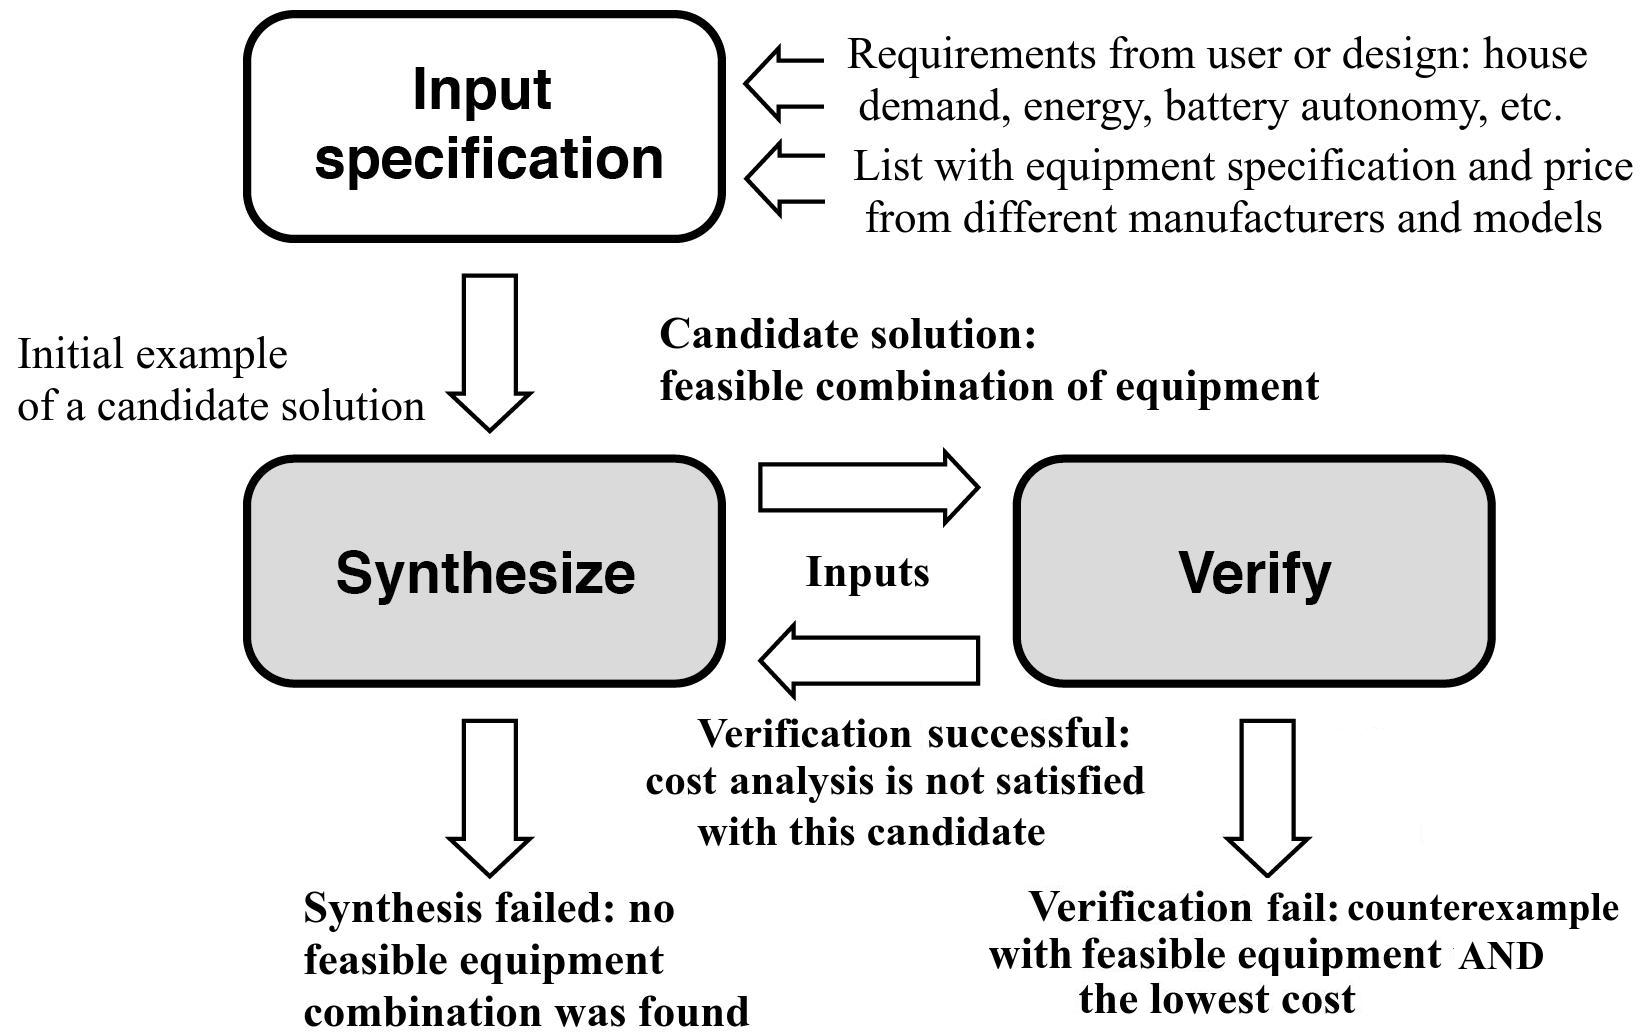
\includegraphics[width=0.75\textwidth]{fig2_rev2.jpg}}
\end{center}
	\caption{CEGIS in PV system sizing.}
	\label{Counter-Example-Guided-Inductive-Synthesis}
\end{figure}

The correctness specification $\sigma$ provided to our synthesizer is of the form $\exists \vec{F}. \forall \vec{x}. \sigma(\vec{x}, \vec{F})$, where $\vec{F}$ ranges over functions, $\vec{x}$ ranges over ground terms, and $\sigma$ is a quantifier-free (QF) formula typically supported by SMT solvers. The ground terms are interpreted over some finite domain $\mathcal{D}$, where $\mathcal{D}$ can be encoded using the SMT's bit-vectors part. Our specification includes house demand, energy, and battery autonomy; we also provide equipment specifications and prices from different manufacturers and models.

In Figure~\ref{Counter-Example-Guided-Inductive-Synthesis}, the phases {\sc Synthesize} and {\sc Verify} interact via a finite set of test vectors {\sc inputs}, which is incrementally updated. Given the correctness specification $\sigma$, the {\sc Synthesize} procedure tries to find an existential witness $\vec{F}$ satisfying the specification $\sigma(\vec{x}, \vec{F})$, for all $\vec{x}$ in {\sc inputs} (as opposed to all $\vec{x} \in \mathcal{D}$). If {\sc Synthesize} succeeds in finding a witness~$\vec{F}$, the latter is a candidate solution to the full synthesis formula, which is passed to {\sc Verify} to check whether it is a proper solution ({\it i.e.}, $\vec{F}$ satisfies the specification $\sigma(\vec{x}, \vec{F})$ for all $\vec{x}\in\mathcal{D}$). If this is the case, then the algorithm terminates.

One may notice that each iteration of the traditional CEGIS loop adds a new input to the finite set $INPUTS$, which is then used for synthesis. Given that the full set of inputs $\mathcal{D}$ is finite because we use bit-vector expressions, the refinement loop can only iterate over a finite number of times. However, {\sc Synthesize} may conclude that no candidate solution obeying $\sigma$ for the finite set $INPUTS$ exists. 

In our CEGIS variant, there exist four differences related to the traditional one: 
(1) there exists no test vector, and every candidate is generated in the {\sc Synthesize} phase and sent to the {\sc Verify} phase; 
(2) if the {\sc Verify} phase is unsuccessful, then a new candidate is generated by {\sc Synthesize} and 
(3) the lower bound of the {\sc Verify} phase is incremented to search for the lowest cost; as a result,
(4) there exists no refinement from the {\sc Verify} phase back to the {\sc Synthesize} phase. In particular, a new counterexample is not added to the {\sc input} set since a failure during the {\sc Verify} phase will only discard a given candidate, which could be feasible in the next iteration with a new lower bound.

%%%%%%%%%%%%%%%%%%%%%%%%%%%%%%%%%%%%%%%%%%%%%%%%%%%%%%%%
\subsection{Sizing Stand-alone Solar PV Systems}
\label{sec:sizing}
%%%%%%%%%%%%%%%%%%%%%%%%%%%%%%%%%%%%%%%%%%%%%%%%%%%%%%%%

A PV system is illustrated in Fig.\ref{fig:blockdiagram}. It employs the PV generator (\textit{panel or an array}), a semiconductor device that can convert solar energy into DC electricity. For night hours or rainy days, we hold \textit{batteries}, where power can be stored and used. The use of batteries as a storage form implies the presence of a \textit{charge controller}~\cite{Hansen}. The PV arrays produce DC, and therefore when the PV system contains an AC load, a DC/AC conversion is required (\textit{inverter}). The \textit{AC load} dictates the behavior of the AC electrical load from the house that will be fed by the system.
%
\begin{figure}[h]
\fbox{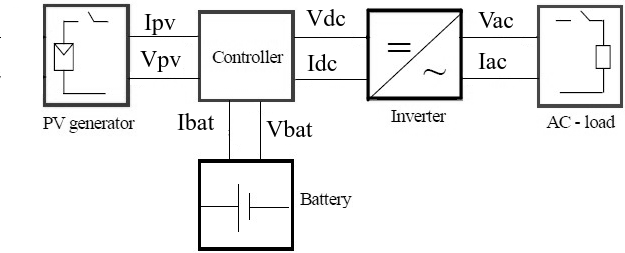
\includegraphics[width=0.8\textwidth]{blockdiagramPVS2_rev}}
\centering
\caption{Block diagram for a typical stand-alone PV system~\cite{Hansen}.}
\label{fig:blockdiagram} 
\end{figure}

The sizing check stage can ensure that the system meets the standard project steps related to the critical period method (worst month) for solar energy system sizing~\cite{Pinho}. It adopts an MPPT (Maximum Power Point Tracking) charge controller, which is the most common in use. 

\textcolor{blue}{In this paper, which audience is targeted to be from the software verification area, we decided to use a higher-level explanation about the PV sizing. The sizing process involves a set of eighteen equations related to the electrical engineering area, which is detailed online \textcolor{red}{I was unable to open this file}\footnote{\url{https://drive.google.com/file/d/1C\_OEo06Or0TrcaysHtYQAP1awa9VNR-T/view?usp=sharing}}. The flowchart pictured in Fig.~\ref{fig:flow} is the overview of the steps that must be taken to size a stand-alone PV system.}
%
\begin{figure}[h]
\fbox{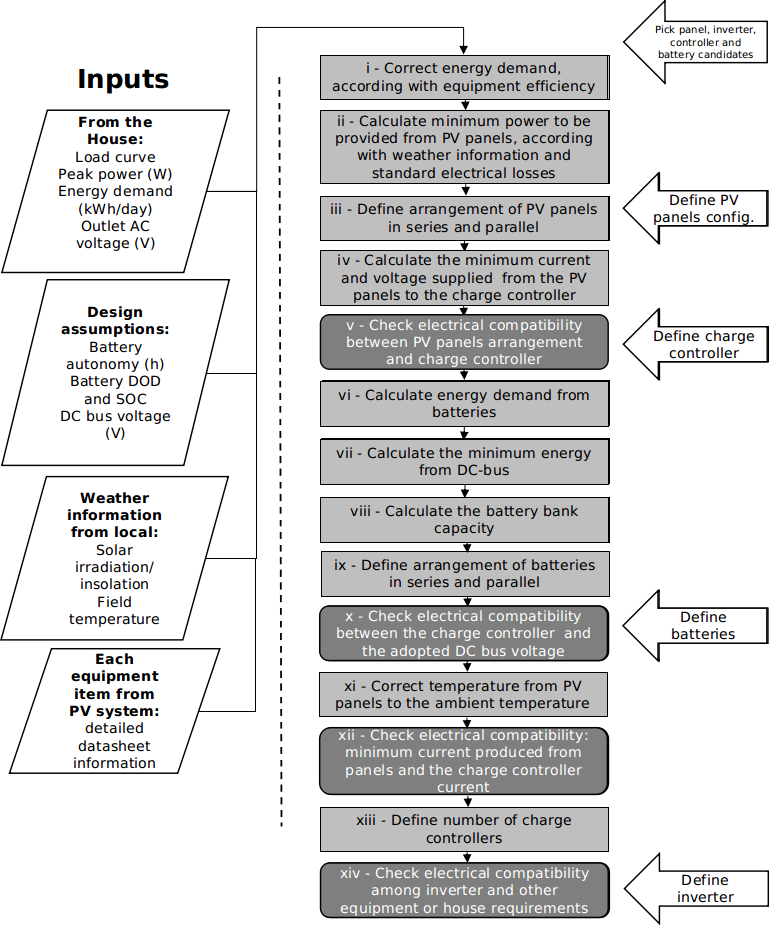
\includegraphics[width=0.9\textwidth]{flowchart}}
\centering
\caption{\textcolor{blue}{High level description of stand-alone PV system sizing process.}}
\label{fig:flow} 
\end{figure}

\textcolor{blue}{On the left side of Fig.~\ref{fig:flow}, we can visualize the needed \textbf{inputs} to size a PV system. There exist requirements from the house to be electrified; in particular, there exist design assumptions, weather information from the targeted local of the PV system deployment, and a possible initial list of equipment to be used, covering all the items listed in Fig.\ref{fig:blockdiagram}. Related to the equipment list, the designer can use a few equipments or a vast one. We can also decide not to adopt the commercial equipment list. However, the result is a PV sizing of specific power, current, or voltage values, and usually just close to original equipment, which can be found in the market. This possibility has the drawback of possible incompatibility among equipment when the real one is bought and deployed.}

\textcolor{blue}{There exist specific steps that aim the calculation of some variables and others related to the electrical compatibility validation among equipment items, both enumerated from \textbf{i} to \textbf{xiv}, as illustrated in Fig.~\ref{fig:flow}; those represent different shades of gray of the rectangle boxes. The start point is usually a candidate list of PV panels, charge controller, battery, and inverter, as indicated at the top of the flowchart. The arrows, on the right side, show a point where some specific item is validated. The diagram does not show the returning location. However, if the candidate item is not compatible with others or does not meet some requirement, it must be changed to follow the indicated flux. The last rectangle box checks the inverter electrical compatibility with the DC-bus voltage, with the required AC voltage from the outlet. Besides, the inverter specified power must be lower than the charge controller power to avoid it from burning by overcharge. At the end of the flowchart, all the items are defined, and the PV sizing is finished.}

\textcolor{blue}{These equations model} the continuous-time behavior of the PV system; they produce real numbers except for the batteries and panels, where real numbers must be converted into integer ones, considering the minimum or maximum according to each equation. The verification and simulation tools need to handle non-linear real arithmetic to produce the correct result. \textcolor{blue}{Our mathematical model uses floating-point arithmetic. It is just an approximation of the real numbers. However, in this work, we are not concerned with calculating the rounding error, which is negligible when considering the size of the physical quantities and the variables adopted~\cite{DBLP:journals/corr/abs-2004-12699}.}

%------------------------------------------------------
\section{Synthesizing Optimal Sizing of Stand-alone Solar Photovoltaic Systems}
%------------------------------------------------------

The best compromise between two objectives makes the optimal sizing of PV systems: \textit{power reliability} and \textit{system cost}~\cite{Alsadi2018}. This study will rely on the critical period solar energy method~\cite{Pinho}, as described in Section~\ref{sec:sizing}. \textcolor{blue}{Our study will use an adapted Life Cycle Cost (LCC) analysis, where the acquisition cost of every item of equipment is considered, plus the installation cost, the operational and maintenance costs}~\cite{Alsadi2018}, given as,
%
\begin{equation}
\label{eq:LCC}
LCC = C_{PV} + C_{bat} + C_{charger} + C_{inv} + C_{installation} + C_{batrep} + C_{PWO\&M}
\end{equation}

\noindent where $C_{PV}$ is the PV array cost, $C_{bat}$ is the initial cost of batteries, $C_{charger}$ is the cost of the charger, $C_{inv}$ is the inverter cost, $C_{installation}$ is the installation cost, $C_{batrep}$ is battery replacement cost at current prices, and $C_{PWO\&M}$ is operation and maintenance costs at current rates. \textcolor{blue}{In this study, we will use a $C_{installation}$ equivalent to 5\% of total equipment cost and a $C_{PWO\&M}$ equal to U\$ 289.64/year according to Amazon State literature data~\cite{Agrener2013}.}

Algorithm~\ref{alg:opt-algorithm} describes our pseudo-code to synthesize stand-alone PV systems using software model checking as a backend verification engine~\cite{DBLP:journals/corr/abs-1909-13139}. The analytical method of optimization was adopted.

 \begin{algorithm}[h]
 \caption{Synthesis algorithm}
 \begin{algorithmic}[1]
 \renewcommand{\algorithmicrequire}{\textbf{Input:}}
 \renewcommand{\algorithmicensure}{\textbf{Output:}}
 \REQUIRE weather data (temperature, solar irradiance); data from panels, controllers, batteries, and inverters; design requirements (load curve, peak demand, load surge power, energy consumption, battery autonomy, AC voltage); design assumptions (SOC, DOD, criteria and objectives for technical and cost analysis)
 \ENSURE FAIL (SAT) with counterexample showing the optimal sizing; SUCCESS (UNSAT), saying that the project has no feasible solution considering the requirements and the list of equipment
 \STATE Initialize variables \\
 \STATE Declare the maximum possible cost $MaxCost$ \\
 \STATE Calculate min possible Cost $MinCost$, based on the equipment list \\
 \FOR {$HintCost=MinCost$ to $MaxCost$} 
 	\STATE Declare non-deterministic variables to select PV Panel, Controller, Battery, and Inverter from list \\
 	\STATE Calculate Steps i and ii of Fig.~\ref{fig:flow} \\
	\STATE Define PV panels arrangement: Step iii of Fig.~\ref{fig:flow} \\
	\STATE Calculate Step iv of Fig.~\ref{fig:flow} \\
	\STATE Enforce electrical compatibility in Step v of Fig.~\ref{fig:flow} with statement \textbf{assume} \\
	\STATE Calculate Steps vi to viii of Fig.~\ref{fig:flow} \\
	\STATE Define battery arrangement according Step ix of Fig.~\ref{fig:flow} \\
	\STATE Enforce electrical compatibility in Step x of Fig.~\ref{fig:flow} with statement \textbf{assume} \\
	\STATE Correct variables to ambient temperature: Step xi of Fig.~\ref{fig:flow} \\
	\STATE Enforce electrical compatibility in Step xii of Fig.~\ref{fig:flow} with statement \textbf{assume} \\
	\STATE Define number of charge controllers: Step xiii of Fig.~\ref{fig:flow}\\
	\STATE Enforce electrical compatibilities in Step xiv of Fig.~\ref{fig:flow} with statement \textbf{assume} and define the inverter \\
	\STATE Non-deterministic variables hold feasible equipment and cost \\
	\STATE $F_{obj} \leftarrow N_{TP}*Panel_{Cost} \, + \, N_{TB}*Battery_{Cost} \, + Controller_{Cost} \, + \, Inverter_{Cost} \, + \, Installation_{Cost} \, + \, batrep_{Cost} \, + \, PWO\&M_{Cost}$ \\
	\STATE Violation check with \textbf{assert}$(F_{obj} > HintCost)$ \\
 \ENDFOR
 \RETURN $(\,)$ 
 \end{algorithmic} 
 \label{alg:opt-algorithm}
 \end{algorithm}

Our synthesis algorithm will synthesize constant values; 
it starts with the input of the manufacturer's data and prices of PV panels, batteries, charge controllers, and inverters. Moreover, we define design (house) requirements and design assumptions. 
%
The \textit{for}-loop started in line $4$ controls the lowest cost of the PV solution. In particular, it begins with a value $MinCost$ and stops when the algorithm finds a feasible solution in which the value breaks the $assertion$ stated in line $18$. If that happens, then our algorithm has found an optimal solution, thereby indicating that the {\sc Verify} phase reached a satisfiable condition (\textit{SAT}). The $MaxCost$ value in line $2$ is just a very high value inserted as a limit to the \textit{for}-loop, that meets one of the following requirements. (1) It will never be reached because the optimal solution will be found first (SAT result); or (2) it will be achieved when the search engine did not find a feasible solution for the optimization (UNSAT result).

Our synthesis algorithm uses non-deterministic variables to choose one specific constant from a given list of PV panels, controllers, batteries, and inverters (line $5$). This procedure ensures that our synthesis engine checks all combinations of items from each equipment, and combines them to assemble a viable (candidate) PV solution, which meets user requirements. A list of forty equipment from ten different manufacturers was provided (as INPUT) to our synthesis engine to allow the choice of every item of PV sizing. Datasheet from each item was necessary to collect technical information. Moreover, the price of each item was obtained from available quotations in the market, and if the currency was not in US dollars, then it was used the exchange rate of the day to convert it to US dollars. All this data is available online \textcolor{red}{I was unable to open this file}\footnote{\url{https://drive.google.com/file/d/1DUtM3Ui\_pU54DmtTXnW1DUcanOcXBVeg/view?usp=sharing}}.

\textcolor{blue}{Next, we use a set of equations to calculate the sizing variables (lines $6$, $7$, $8$, $10$, $11$, $13$, $15$). The statements \textit{assume} (lines $9$, $12$, $14$, and $16$) ensures compatibility of the items chosen from the list of equipment: the {\sc Verify} phase uses only items (among all the possible ones) that satisfy the statements of those lines. Line $12$ is for the battery bank. Lines $9$ and $14$ are the charge controller voltage check. Line $16$ does the inverter check and ensures the power demand and the surge power of the inverter. Therefore, our synthesis algorithm reaches line $17$ with one feasible solution, and the cost of that solution is calculated in $F_{obj}$ (line $18$). This cost is the equivalent to Eq.~\eqref{eq:LCC}.}

If our algorithm does not find a feasible solution among the item of equipment that was provided for our {\sc Synthesize} phase, then the result is unsatisfiable (\textit{UNSAT}). In particular, the program finishes without finding a solution, indicating that it was unable to combine the specific items of equipment to create a feasible solution. 
%
The main challenge for the {\sc Synthesize} phase is to find a feasible candidate solution for the constraints and user requirements. The problem for the {\sc Verify} phase is to find the lowest acquisition cost from a list of equipment and components provided by the {\sc Synthesize} phase. 
%
Note that the process described here is completely automated and that validation is performed by our {\sc Verify} phase to ensure that the solution is sound.
The verification engines transform the Algorithm~\ref{alg:opt-algorithm} into the Boolean expressions that are passed to the solver to verify ($C \wedge \neg P$), as described online\footnote{\url{https://drive.google.com/file/d/1Q_hlgUt6AWrNeOtxhFlIpW4P4OPrPyIA/view?usp=sharing}}.

%---------------------------------------------------------------------------
\section{Results and Discussion}
%---------------------------------------------------------------------------
%---------------------------------------------------------------------------
\subsection{Description of the Case Studies}
%---------------------------------------------------------------------------

The proposed synthesis approach was evaluated in seven stand-alone PV system case studies.
These case studies were defined based on the usual electrical load found in riverside communities in the Amazonas State, Brazil~\cite{TrindadeCordeiro19,Agrener2013}, except for case 7, which was idealized to support a few lamps and a 12k BTUs air-conditioner solution. 
Here we report each case study as a 4-tuple \textit{\{power peak (W); power surge (W); energy consumption (Wh/day); battery autonomy (hours)\}} as follows:
\textbf{1:} \{342; 342; 3,900; 48\}; \textbf{2:} \{814; 980; 4,880; 48\}; \textbf{3:} \{815; 980; 4,880; 12\}; \textbf{4:} \{253; 722; 3,600; 48\}; \textbf{5:} \{263; 732; 2,500; 48\}; \textbf{6:} \{322; 896; 4,300; 48\}; \textbf{7:} \{1,586; 2,900; 14,000; 48\}. This 4-tuple represents the Algorithm~\ref{alg:opt-algorithm} inputs. For all cases, an estimated load curve (kWh) was defined based on the electronics consumers in each house. Our synthesis algorithm was fed with data and costs of forty equipment items from ten different manufacturers of PV systems. 
%
Three \textcolor{blue}{state-of-the-art} verifiers, CBMC\footnote{Command-line: \$ cbmc -\phantom{}-unwind 100 file.c -\phantom{}-trace} v5.11 with MiniSat 2.2.1~\cite{Kroening}, ESBMC\footnote{Command-line: \$ esbmc filename.c -\phantom{}-incremental-bmc -\phantom{}-boolector} v6.0.0~\cite{esbmc2018} with the Boolector 3.0.1 solver~\cite{Brummayer}, and CPAchecker\footnote{Command-line: \$ scripts/cpa.sh -heap 64000m -config config/bmc-incremental.properties -spec config/specification/sv-comp-reachability.spc file.c} v1.8~\cite{Beyer2011} with MathSAT 5.5.3~\cite{mathsat5}, were used as verification engines to compare the proposed approach effectiveness and efficiency. 

%---------------------------------------------------------------------------
\subsection{Optimization/Simulation Tools and Assumptions}
%---------------------------------------------------------------------------
Concerning the off-the-shelf optimization/simulation tools, only HOMER Pro performs an off-grid system with battery backup analysis and includes economical analysis. Here we used HOMER Pro version $3.13.1$ as a state-of-the-art optimization tool for comparison purposes. In particular, HOMER Pro has the following characteristics:
(a) it is available only for MS-Windows, its annual standard subscription costs US\$ $504.00$~\cite{HOMER}; 
(b) it has two optimization algorithms: one algorithm simulates all of the feasible system configurations defined by the search space, and additionally, a proprietary derivative-free algorithm to search for the least-costly system;
(c) it does not have LCC cost in its reports, only Net Present Cost (NPC); however, we can obtain LCC from NPC; 
(d) the optimization analysis defines a load curve and temperature according to data collected from online databases. However, to allow a correct comparison, the curve load and the temperature were defined the same as our synthesis approach; 
(e) it does not have a charge controller. During the tests, we have chosen the ``load-following'' option, which produces enough power to meet the demand~\cite{HOMER} and (usually) presents a non-overestimated solution; 
(f) it was assumed 95\% availability of the PV system. By definition, ``availability'' is the percentage of time at which a power system can feed the load requirements~\cite{Khatib2014}. For an ordinary house electrical load, 95\% is considered acceptable;
(g) it was assumed a string of two batteries to match the voltage of the system of $24$ V DC, which was used for our automated synthesis tool; 
(h) it was included a generic flat-plate PV of $1$ kW and generic lead-acid batteries of $1$ kW ($83.4$ Ah capacity). During run-time, HOMER decides the size in kW of each one based on feasibility and lower cost.

In order to validate and compare the optimal sizing solution produced by our approach and by HOMER Pro, we use a simulation tool, called PVsyst version $6.86$~\cite{PVsyst}, with plenty of commercial equipment in its data bank. We have considered a comparison for an entire year's weather data of simulation to guarantee that the proposed sizing meets the electrification requirements. PVsyst is a PC software package developed by a Swiss company used for the study, sizing, simulation, and data analysis of solar PV systems. PVsyst contains design, sizing, 3D shading scene, simulation, grid, and off-grid features. It uses comprehensive irradiation data from Meteonorm\footnote{https://meteonorm.com/en/}, and aging analysis~\cite{PVsyst2017}. However, it does not perform optimization; therefore, PVsyst needs the system sized to validate it. Furthermore, PVsyst does not have commercial inverter equipment and, as a result, does not consider surge power demand as the ones produced by air conditioners and refrigerators for a few seconds. PVsyst is a commerical software with $30$-day test possibility and runs only in MS-Windows.

%---------------------------------------------------------------------------
\subsection{Objectives and Setup}
%---------------------------------------------------------------------------

Our evaluation aims to answer three experimental goals: [EG1] \textbf{(soundness)} Does our automated synthesis approach provide correct results?; [EG2] \textbf{(performance)} How do the software verifiers compare to each other for synthesizing PV systems?; and [EG3] \textbf{(state-of-the-art)} how does our formal synthesis tool compare to a specialized simulation tool?

All experiments regarding the verification tools were conducted on an otherwise idle Intel Xeon CPU E5-4617 ($8$-cores) with $2.90$ GHz and $64$ GB RAM, running Ubuntu $16.04$ LTS $64$-bits. For HOMER Pro, we have used an Intel Core i5-$4210$ ($4$-cores) with $1.7$ GHz and $4$ GB RAM running Windows 10. The ideal scenario would be to use the same hardware configuration for the experiments. However, we faced restrictions concerning the license for the HOMER Pro tool; besides, we did not have the autonomy to change the Linux VM machine installed in the servers of our university due to the internal policy. This has an impact on performance, which is less favourable to HOMER Pro. PVsyst used the same configuration as HOMER Pro. We perform the experiments with a predefined \textit{time out} of $660$ minutes.


%The hardware platform was not the same because of the availability of the machines; 


%---------------------------------------------------------------------------
\subsection{Results}
%---------------------------------------------------------------------------

The results are presented in Table~\ref{tab1}. 
%
\begin{table}
\caption{Case studies and results: optimization of stand-alone PV systems.}\label{tab1}
\begin{scriptsize}
\begin{tabular}{c|c|c|c|c}
\hline
\hline
Tools & \makecell{CBMC 5.11 \\(MiniSat 2.2.1)}& \makecell{ESBMC 6.0.0 \\(Boolector 3.0.1)}& \makecell{CPAchecker 1.8\\(MathSAT 5.5.3)}& HOMER Pro 3.13.1\\
\hline
\hline
Specification & Result & Result & Result & Result \\
\hline
\makecell{\textbf{Case Study 1}\\Peak:342W\\Surge:342W \\E:3,900Wh/day\\Autonomy:48h} & OM & \makecell{SAT (620 min) \\NTP:6$\times$330W (2P-3S)\\NBT:16$\times$105Ah (2S-8P)\\Controller 35A/145V\\Inverter 700W/48V\\LCC: US\$ 10,214.04} & \makecell{SAT (548 min) \\NTP:6$\times$330W (2P-3S)\\NBT:16$\times$105Ah (2S-8P)\\Controller 35A/145V\\Inverter 700W/1600W/48V\\LCC: US\$ 10,214.04} & \makecell{(Time: 0.33 min)\\2.53 kW of PV\\NBT:12$\times$83.4Ah (2S-6P)\\0.351kW inverter\\LCC: US\$ 7,808.04}\\
\hline
\makecell{\textbf{Case Study 2}\\Peak:814W\\Surge:980W\\E:4,880Wh/day\\Autonomy:48h} & OM & TO & TO & \makecell{(Time: 0.18 min)\\3.71 kW of PV\\NBT:20$\times$83.4Ah (2S-10P)\\0.817kW inverter\\LCC: US\$ 12,861.75} \\
\hline
\makecell{\textbf{Case Study 3}\\Peak:815W\\Surge:980W\\E:4,880Wh/day\\Autonomy:12h} & OM & \makecell{SAT (63 min) \\NTP:14$\times$150W (7P-2S)\\NBT:6$\times$105Ah (2S-3P)\\Controller 35A/145V\\Inverter 1,200W/48V\\LCC: US\$ 9,274.07} & TO & Not possible \\
\hline
\makecell{\textbf{Case Study 4}\\Peak:253W\\Surge:722W\\E:3,600Wh/day\\Autonomy:48h} & OM & \makecell{SAT (147 min) \\NTP:6$\times$330W (2P-3S)\\NBT:16$\times$105Ah (2S-8P)\\Controller 35A/145V\\Inverter 280W/48V\\LCC: US\$ 9,678.63} & \makecell{SAT (605 min) \\NTP:6$\times$330W (2P-3S)\\NBT:16$\times$105Ah (2S-8P)\\Controller 35A/145V\\Inverter 280W/48V\\LCC: US\$ 9,678.63} & \makecell{(Time: 0.23 min)\\2.42 kW of PV\\NBT:12$\times$83.4Ah (2S-6P)\\0.254kW inverter\\LCC: US\$ 7,677.95}\\
\hline
\makecell{\textbf{Case Study 5}\\Peak:263W\\Surge:732W\\E:2,500Wh/day\\Autonomy:48h} & OM & \makecell {SAT (36.70 min) \\NTP:4$\times$330W (2S-2P)\\NBT:14$\times$80Ah (2S-7P)\\Controller 35A/145V\\Inverter 280W/24V \\LCC: US\$ 8,900.70} & \makecell {SAT (254.25 min) \\NTP:4$\times$330W (2S-2P)\\NBT:14$\times$80Ah (2S-7P)\\Controller 35A/145V\\Inverter 280W/24V \\LCC: US\$ 8,900.70} & \makecell{(Time: 0.18 min)\\1.59 kW of PV\\NBT:10$\times$83.4Ah (2S-5P)\\0.268kW inverter\\LCC: US\$ 6,175.57} \\
\hline
\makecell{\textbf{Case Study 6}\\Peak:322W\\Surge:896W\\E:4,300Wh/day\\Autonomy:48h} & OM & \makecell {SAT (380.93 min) \\NTP:6$\times$320W (2P-3S)\\NBT:18$\times$105Ah (2S-9P)\\Controller 35A/145V\\Inverter 400W/24V \\LCC: US\$ 10,136.61} & TO & \makecell{(Time: 0.22 min)\\3.15 kW of PV\\NBT:14$\times$83.4Ah (2S-7P)\\0.328kW inverter\\LCC: US\$ 9,112.45} \\
\hline
\makecell{\textbf{Case Study 7}\\Peak:1,586W\\Surge:2,900W\\E:14,000Wh/day\\Autonomy:48h} & OM & UNSAT (0.48 min) & TO & \makecell{(Time: 0.20 min)\\12.5 kW of PV\\NBT:66$\times$83.4Ah (2S-33P)\\1.60kW inverter\\LCC: US\$ 41,878.11} \\
\hline
\hline
\end{tabular}
\\Legend: OM = out of memory; TO = time out; IF = internal failure; E = energy;    NTP = total number of panels, NBtotal = total number of batteries, NPS = number of panels in series; NPP = number of panels in parallel, NBS = number of batteries in series; NBP = number of batteries in parallel; LCC = Life Cycle Cost.
\end{scriptsize}
\end{table}
%
The violation (SAT result) indicated all over the Table~\ref{tab1} 
is the $assert$ of the line $18$ in Algorithm~\ref{alg:opt-algorithm} and indicates that an optimal solution was found.
Here, CBMC was unable to produce any conclusive result. \textit{Out of memory} situations occurred in all case studies.

CPAchecker was able to synthesize optimal sizing in three out of the seven case studies (cases $1$, $4$, and $5$): the result was produced within the time limit, which varied from $4$ to $9$ hours. 
Fig.~\ref{fig:CPAoptc1} illustrates the result of case $5$ with the optimal sizing appearing on the left side as the integer $3$ for the solar panel (which is the Canadian CS6U-330P model of $330$ W from the manufacturer Victron Energy), battery $0$ refers to the model 12MF80 of $80$ Ah from Moura, charge controller $0$ refers to the model 35A-145V MPPT from Victron Energy. The inverter number $2$ refers to the Epever model IP350-11 of $280$ W (nominal power) and $750$ W of surge power. The variables NTP, NPS, NPP, NBS, NBP, and NBTotal, also presented in the counterexample, shows the number of panels and batteries and how they are connected.
Case studies $2$, $3$, $6$, and $7$ led to a \textit{time out} result in CPAchecker, i.e., it was not solved within $11$ hours.  
%
\begin{figure}[h]
\fbox{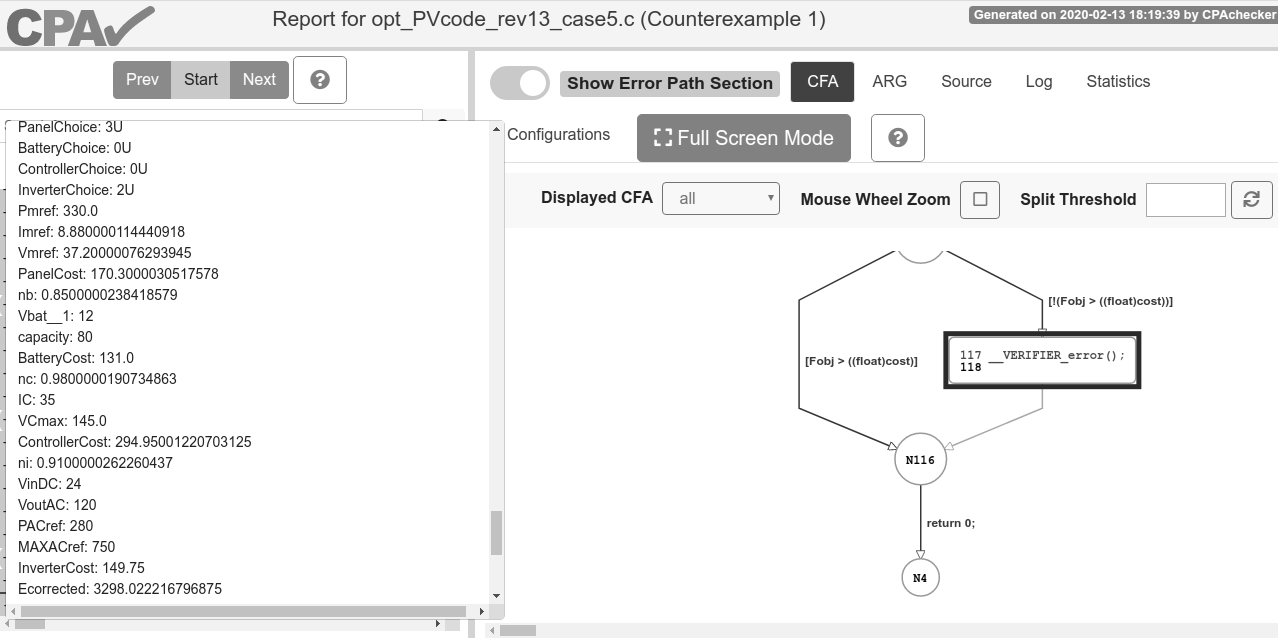
\includegraphics[width=0.9\textwidth]{CPA_opt_c5.png}}
\centering
\caption{Counterexample generated by CPAchecker after validation of case $5$.}
\label{fig:CPAoptc1}
\end{figure}

Here we used ESBMC in incremental mode with Boolector; ESBMC was able to reach the optimal sizing of case studies $1$, $3$, $4$, $5$, and $6$ with a FAIL/ SAT response, varying from $36$ minutes to $10$ hours. ESBMC, with this configuration, was unable to obtain an optimal solution in cases $2$ and $7$. Case $2$ produced a \textit{time out}. Moreover, case $7$ resulted in a UNSAT result, i.e., ESBMC was unable to provide a feasible solution. However, this is not a bug, and it means that the available list of equipment can not produce a feasible solution that satisfies electrical compatibility or design requirements. This UNSAT situation was reached in less than one minute. These experimental results answer the \textit{EG2}.

HOMER Pro was able to evaluate six case studies (cases $1$, $2$, $4$, $5$, $6$, and $7$) under $30$ seconds; it was much faster than the proposed automated synthesis tool (cf.~\textit{EG3}). Case study $3$ could not be simulated since HOMER Pro does not have the battery autonomy adjustment feature, i.e., the tool always tries to feed the given load with electricity $365$ days/year. Some HOMER Pro drawbacks were also noted. (1) System equipment does not include an explicit charge controller. HOMER Pro includes a controller automatically to simulate the charge/discharge of batteries and to meet the load requirement. However, without costs or even with electrical characteristics such as maximum current and voltage, which are common during PV sizing. (2) HOMER Pro requires the inclusion of some battery specification to initiate optimization; however, it does not change the electrical specifications during simulation; the results presented are multiples of the original battery type suggested by the user. For example, it was started with a $83.4$ Ah lead-acid battery, and during simulation, HOMER Pro did not try to use other capacities or types. (3) HOMER Pro does not present the optimal solution in terms of connections of PV panel arrays, just the total in terms of power, i.e., it presents neither the models and the power of each PV panel nor the total of panels in series or parallel.

The authors have real PV systems deployed since June $2018$ in a riverside community in the State of Amazonas, Brazil, GPS coordinates 2$^{o}$44'50.0"S 60$^{o}$25'47.8"W, with demands of case studies $1$, $4$, $5$, and $6$, always with a $3$ $\times$ $325$ W ($3$S, total $975$ W) panels and $4$ $\times$ $220$ Ah ($2$S-$2$P $= 440$ Ah) lead-acid batteries.

%%%%%%%%%%%%%%%%%%%%%%%%%%%%%%%%%%%%%%%%%%%%%%%%%%%%%%%%%%%%%%%%%%%%
\subsection{Comparison Between Formal Synthesis and HOMER Pro}
%%%%%%%%%%%%%%%%%%%%%%%%%%%%%%%%%%%%%%%%%%%%%%%%%%%%%%%%%%%%%%%%%%%%
If we compare the results of the formal synthesis against those of HOMER Pro, we observed some distinct results in terms of the technical solution and cost (cf. Table~\ref{tab1}). Concerning the performance, there exists a vast difference in favor of HOMER Pro that obtained the results in considerably less time: few seconds in the opposite of an average of $4$ hours for the automated synthesis technique.
%
Particularly in the case of LCC, the cost varied from $11$\% to $44$\%, producing a higher estimation from the automated synthesis technique. However, considering that the cost of individual items of each database used to compose the optimal design is not the same among the tools, it is plausible to obtain distinct results.

On the one hand, concerning the PV panels sizing, the results presented by the automated synthesis were smaller in terms of power than the ones produced by the simulation tool. The difference varied from $19$\% to $65$\%. On the other hand, concerning the battery bank, the results were smaller in terms of capacity for HOMER Pro. The difference was between $34$\% to $68$\%. The mathematical models are different and particular parameters can be tuned for each technique, and that can justify the difference, which was presented in all the case studies.

Those discrepancies are not easy to address without some real systems validation. However, we use the simulation software PVsyst to validate the optimal sizing produced, as shown in Table~\ref{tab2}. Note that PVsyst has a pre-sizing feature, which presents a minimum recommended sizing of PV panels and batteries (only), but without using manufacturers' data or models for it. This feature was used as reference mainly with HOMER Pro, where there exists no equipment brands or models (only power and capacities specification). PVsyst was used with the field-deployed and the formal synthesis sizing solutions, where brands and models were simulated in PVsyst according to the sized system.

\begin{table}
\caption{Optimal sizing validation with PVsyst.}
\label{tab2}
\begin{scriptsize}
\begin{tabular}{c|c|c|c|c}
\hline
\hline
CS & \makecell{PVsyst\\(pre-sizing)}& \makecell{Field\\deployed\\validation}& \makecell{Formal synthesis\\sizing\\validation}& \makecell{HOMER Pro\\sizing\\validation}\\
\hline
\hline
CS 1 & \makecell{P= 1,166 W\\B= 381 Ah\\(minimum)} & \makecell{Not correct sizing \\Avail. $<$ 95\%\\(91.06\%)} & \makecell{No error found \\100\% of avail.} & \makecell{No error found\\Panels oversized in 2.16 $\times$\\Batteries oversized in 1.39 $\times$}\\
\hline
CS 2 & \makecell{P= 1,482 W\\B= 478 Ah\\(minimum)} & \makecell{NA\\There exists no real PV system\\available for comparison} & \makecell{NA \\(TO result\\in Table~\ref{tab1})} & \makecell{No error found\\Panels oversized in 2.6 $\times$\\Batteries oversized in 1.74 $\times$}\\
\hline
CS 3 & \makecell{Not possible to \\simulate\\(autonomy $<$ 24h)} & \makecell{NA\\There exists no real PV system\\available for comparison} & \makecell{Only technique that\\produced solution} & \makecell{NA\\(autonomy $<$ 24h)}\\
\hline
CS 4 & \makecell{P= 1,078 W\\B= 354 Ah\\(minimum)} & \makecell{No error found \\95.76\% of avail.} & \makecell{No error found \\97.37\% of avail.} & \makecell{No error found\\Panels oversized in 2.24 $\times$\\Batteries oversized in 1.41 $\times$}\\
\hline
CS 5 & \makecell{P= 823 W\\B= 268 Ah\\(minimum)} & \makecell{No error found \\100\% of avail.} & \makecell{No error found \\100\% of avail.} & \makecell{No error found\\Panels oversized in 1.93 $\times$\\Batteries oversized in 1.56 $\times$}\\
\hline
CS 6 & \makecell{P= 1,299 W\\B= 421 Ah\\(minimum)} & \makecell{Not correct sizing \\Avail. $<$ 95\%\\(85.65\%)} & \makecell{No error found \\100\% of avail.} & \makecell{No error found\\Panels oversized in 2.42 $\times$\\Batteries oversized in 1.38 $\times$}\\
\hline
CS 7 & \makecell{P= 4,263 W\\B= 1,384 Ah\\(minimum)} & \makecell{NA\\There exists no real PV system\\available for comparison} & \makecell{NA \\(UNSAT result\\in Table~\ref{tab1})} & \makecell{No error found\\Panels oversized in 2.9 $\times$\\Batteries oversized in 1.99 $\times$}\\
\hline
\hline
\end{tabular}
\\Legend: CS = case study; NA = sizing not available for validation; B = batteries capacity; P = panels power; Avail.= Availability (expected of 95\% or greater as a design requirement).
\end{scriptsize}
\end{table}

Each simulation with PVsyst took $4$ seconds. We were unable to validate case study $3$ using PVsyst since the battery autonomy is less than 24 hours, and only the proposed synthesis technique can perform the optimal sizing (PVsyst and HOMER Pro are limited for a $24$ h minimum). Case studies $2$ and $7$ had only HOMER Pro sizing validation, because there exists no deployed equivalent system in the field, and the synthesis technique did not present a solution due to \textit{time out} and internal failures in the underlying verification engine. %(our technique presented a \textit{time out} in case study $2$ and an \textit{UNSAT} in the case study $7$).

Overall, those comparisons among our approach, the optimization software, and the deployed systems, with validation through simulation tool, show that the synthesis solution is sound and complete, which answers \textit{EG1} and {EG3}.

HOMER Pro suggests a value in kW for the inverters that are very close to the maximum load of every case study, but it is not a commercial value. The proposed synthesis tool, however, presents inverters that are commercial and can be obtained off-the-shelf. Moreover, our synthesis approach considers surge power demand from the house, which is not considered by HOMER Pro or PVsyst. This feature is a definite advantage of the formal synthesis method. HOMER Pro does not include charge controllers as a specific item of equipment in its mathematical model; only the synthesis tool presents a commercial controller and includes it during the cost analysis. The formal synthesis method, therefore, presents more reliable results than HOMER Pro.

In summary, our synthesis technique can present a solution that is far more detailed and closer to commercial conditions than the solution presented by HOMER Pro. In particular, the automated synthesis method can provide all the details of every component of a PV system solution, with complete electrical details from the manufacturer datasheet, including the model of the component, nominal current, and voltage. In this respect, even the name of the manufacturer can be cited (in Table~\ref{tab1}, it was removed to avoid unauthorized advertising). Moreover, the validation through PVsyst simulation, using the PV sizing produced by HOMER Pro and our synthesis approach, shows that our results are feasible and not as oversized as HOMER Pro results, mainly concerning PV panels.

\textcolor{blue}{Worth to mention that an optimal solution from a tool is not necessarily the same optimal from other tool, mainly when the data base of equipment items (with different costs) are not the same. Therefore the comparison must take this issue into account.} 

%---------------------------------------------------------------------------
\subsection{Threats to validity} 
%---------------------------------------------------------------------------
We have reported a favorable assessment of the proposed method. Nevertheless, we have also identified four threats to the validity of our results that constitute future work. First, improvement of the power reliability analysis: to include loss of load probability or loss of power supply probability, which can make the analysis more accurate. Second, improvement of the system cost analysis by including operational and maintenance costs to the adopted LCC analysis. Third, increase the equipment and manufacturers database: this will increase the optimization complexity, but the result will also allow improved sizing. Lastly, the underlying software verifiers employed here perform bit-precise verification based on the Floating-Point (FP) theory. We could use a real arithmetic strategy to tackle these equations; however, in this study, we have exploited the FP arithmetic, which is an approximation of the real one. 
%------------------------------------
\section{Conclusions} 
%------------------------------------
Our novelty relies on a practical approach to pursue the optimal solution of PV systems using contemporary formal methods. The use of formal synthesis to design PV systems has no precedent in literature; we show that the results of our approach, using seven case studies, are promising. Our synthesis tool can present a solution, which is far more detailed and closer to the commercial reality than the solution presented by the commercial tool. In particular, the battery autonomy feature, together with the details of every component of a PV system solution, is an advantage for our synthesis approach. These technical details are essential for the owner of the PV system since the industry demands proximity between the result presented by optimization tools and the items of equipment for solar systems available on the market. It is worth mentioning that our synthesis technique was developed and used open-source software verifiers and the environment, in contrast to the optimization and simulation tools used in this work. We have also observed that state-of-the-art software verifiers are doing an excellent job of solving hard verification conditions based on the underlying SAT/SMT solvers. Lastly, the use of data from real deployed systems in Brazil and the validation through PVsyst was essential to validate the comparison. For future work, %we will investigate the application of probabilistic programming within our research for the trade-off between performance and precision.
\textcolor{blue}{now that we proved that our technique has a promising result for PV system sizing optimization, our focus will be the improvement with the search mechanism used in the {\sc Verify} phase of our synthesis technique, in order to speed up the time to response. Using binary search or even a solver that is specific to perform optimization with model checking as $\nu Z$.}

%
% ---- Bibliography ----
% BibTeX users should specify bibliography style 'splncs04'.
% References will then be sorted and formatted in the correct style.
%
\bibliographystyle{splncs04}
\bibliography{trindadeThesis}
%
\end{document}
%\subsection{Design and Simulation of Solar PV systems}
%The design and validation of a PV system can be done by hand or with the aid of a software tool. In order to address different aspects of the PV system design, there are various software tools available in the literature~\cite{Rajanna,Rawat}.
%public domain and commercial software available for the PV market. 
%According to \cite{Brooks}, t
%%%%%%%%%%
%
%The capabilities of tools available in the literature range from simple solar resource and %energy production estimation, %to site survey and system design tools,
%to complex financial analysis and project optimization. At this study, the commercial simulation tool HOMER PRO was selected to be used at the case studies in order to be compared with the automated verification tools.
